\section{Objects and defects}
StarGen script supports multiple astronomical objects such as stars, galaxies, clusters, and moving objects. Apart from galaxies, all mentioned objects have two types of appearances: point and streak. In the script, we also generate defects such as hot pixels and three types of cosmic rays. Here we will explain how each object, in a morphological sense, is generated and show some examples. 

\subsection{Point}
Generation of point is performed using two dimensional Gaussian function with the following formula: 
\begin{equation} \label{eq:gauss}
    f(x,y) = \frac{1}{2 \pi \sigma^2} \cdot \exp{\left( - \frac{1}{2} \left( \frac{(x - x_0)^2 + (y - y0)^2 }{2 \sigma^2} \right) \right)}
\end{equation}
where $x_0$, $y_0$ are coordinates of the point and $\sigma$ is the standard deviation computed from the fwhm of the Gaussian. 

The point is generated by the following process. A blank image is created and the Gaussian function is used to generate a point on the image using the position and fwhm of the object. The values of the image are then normalized to interval <0,1> and multiplied by the brightness of the object. Poisson noise is applied and image values are clipped to the interval <0,65535>. This image of the object is then added to the input image. If we are generating only one object per frame, then the input image is blank and we could just return the image of the object. However, if we are generating frames with multiple objects then we need to add the new point to the input image. 

To compare the performance of our generator to real data we show the 3D profile of the real point and our generated point in a side-by-side view in the Figure \ref{fig:point3D}

\begin{figure}[H]
\centering
    \begin{subfigure}[t]{.4\textwidth}
        \centering
        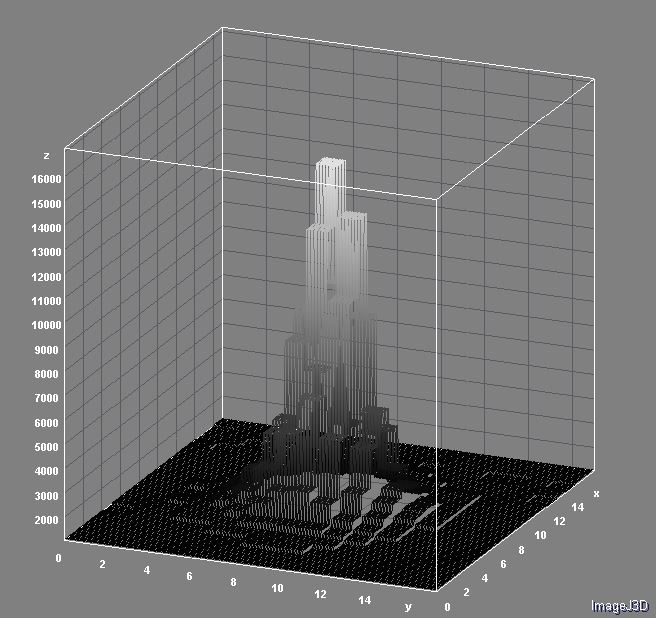
\includegraphics[width=\textwidth]{images/realPoint3D.JPG}
        \caption{3D profile of the real point source.}
        \label{fig:point3D1}
    \end{subfigure}
    \begin{subfigure}[t]{.4\textwidth}
        \centering
        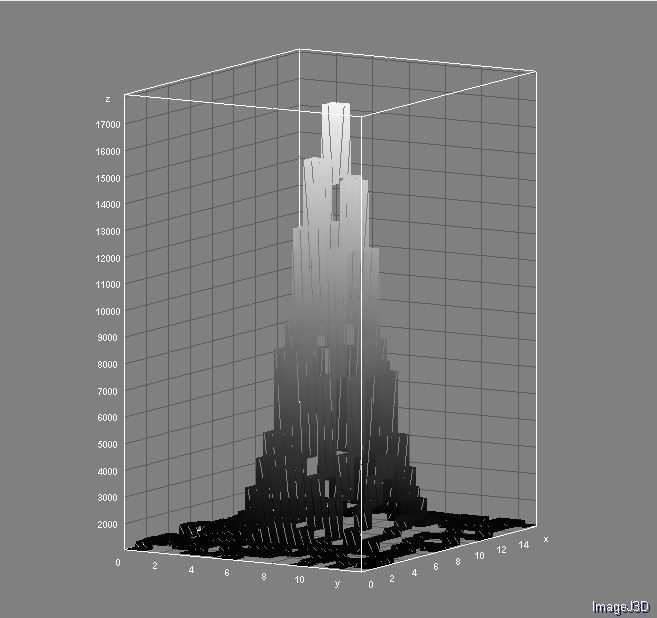
\includegraphics[width=\textwidth]{images/synpoint3D.JPG}
        \caption{3D profile of the synthetic point source.}
        \label{fig:point3D2}
    \end{subfigure}

    \caption{Comparison of 3D profiles between real and synthetic point source.}
    \label{fig:point3D}
\end{figure}

With point source, there aren't many parameters other than $fwhm$ and $brightness$ that can be configured. In the Figure \ref{fig:pointfwhm} we show generated images with various values of fwhm of the Gaussian function. 


\begin{figure}[!h]
\centering
    \begin{subfigure}{.23\textwidth}
        \centering
        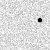
\includegraphics[width=\textwidth]{images/fwhm2.png}
        \caption{fwhm = 2.}
        \label{fig:pointfwhm2}
    \end{subfigure}
    \begin{subfigure}{.23\textwidth}
        \centering
        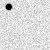
\includegraphics[width=\textwidth]{images/fwhm3.png}
        \caption{fwhm = 3.}
        \label{fig:pointfwhm3}
    \end{subfigure}
    \begin{subfigure}{.23\textwidth}
        \centering
        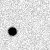
\includegraphics[width=\textwidth]{images/fwhm4.png}
        \caption{fwhm = 4.}
        \label{fig:pointfwhm4}
    \end{subfigure}
    \begin{subfigure}{.23\textwidth}
        \centering
        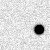
\includegraphics[width=\textwidth]{images/fwhm5.png}
        \caption{fwhm = 5.}
        \label{fig:pointfwhm5}
    \end{subfigure}

    \caption{Generated images of point source with different values of fwhm.}
    \label{fig:pointfwhm}
\end{figure}


\subsection{Streak}
The streak source is generated using multiple overlapping two-dimensional Gaussian functions with the same Formula \ref{eq:gauss}. The process of the generation is similar to the point source but other parameters other than $\sigma$ and $brightness$ need to be taken into an account. The rotation of the streak relative to the positive x-axis is determined by parameter $alpha$. And half-length of the streak is set by $length$. Figure \ref{fig:streak3D} shows the comparison of the real and synthetic 3D profile of the streak source. 


\begin{figure}[!h]
\centering
    \begin{subfigure}[t]{.4\textwidth}
        \centering
        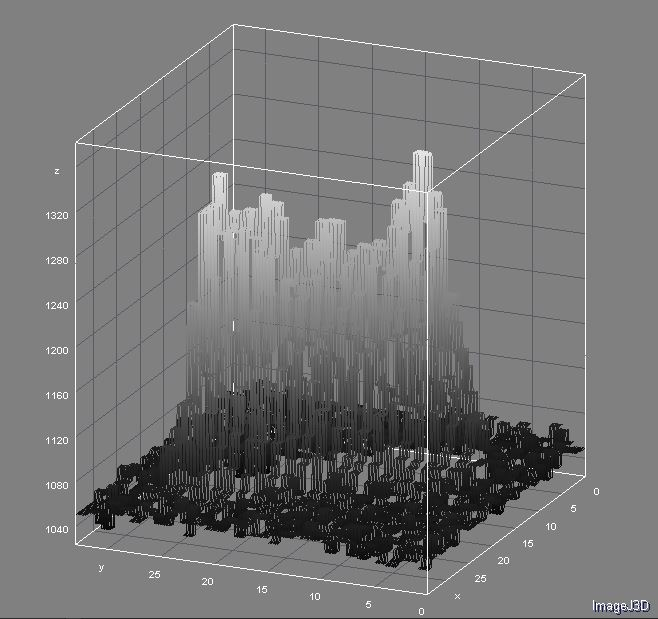
\includegraphics[width=\textwidth]{images/realStreak3D.JPG}
        \caption{3D profile of the real streak source.}
        \label{fig:streak3D1}
    \end{subfigure}
    \begin{subfigure}[t]{.4\textwidth}
        \centering
        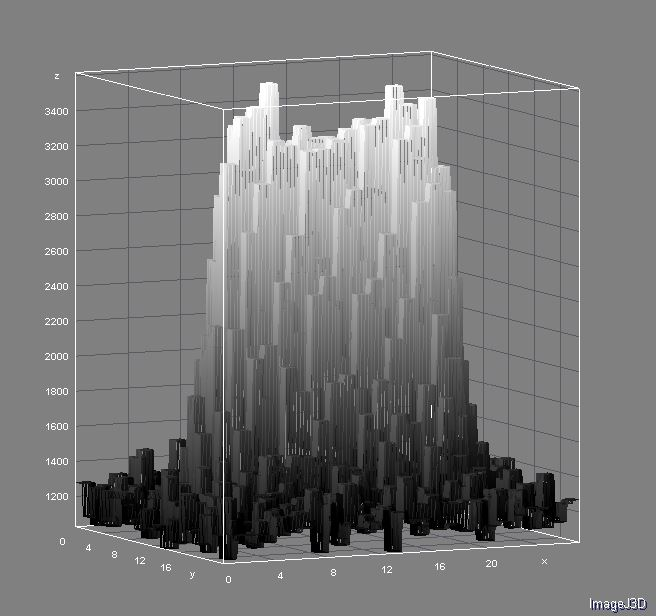
\includegraphics[width=\textwidth]{images/synStreak3D.JPG}
        \caption{3D profile of the synthetic streak source.}
        \label{fig:streak3D2}
    \end{subfigure}

    \caption{Comparison of 3D profiles between real and synthetic streak source.}
    \label{fig:streak3D}
\end{figure}

In the Figure \ref{fig:pointfwhm} we have shown how fwhm affects the size of the point source. With streak source, the fwhm affects its width. As the name suggests, the length determines how long the streak is and alpha describes its rotation. Examples of generated streak sources with different settings of parameters are shown in the Figure \ref{fig:streakspar}. 

\begin{figure}[!h]
\centering
    \begin{subfigure}{.23\textwidth}
        \centering
        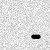
\includegraphics[width=\textwidth]{images/streakA.png}
        \caption{fwhm = 2, alpha = 0, length = 3.}
        \label{fig:streakA}
    \end{subfigure}
    \begin{subfigure}{.23\textwidth}
        \centering
        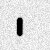
\includegraphics[width=\textwidth]{images/streakB.png}
        \caption{fwhm = 3, alpha = 90, length = 5.}
        \label{fig:streakB}
    \end{subfigure}
    \begin{subfigure}{.23\textwidth}
        \centering
        
\includegraphics[width=\textwidth]{images/streakC.png}
        \caption{fwhm = 4, alpha = 135, length = 7.}
        \label{fig:streakC}
    \end{subfigure}
    \begin{subfigure}{.23\textwidth}
        \centering
        
\includegraphics[width=\textwidth]{images/streakD.png}
        \caption{fwhm = 5, alpha = 45, length = 9.}
        \label{fig:streakD}
    \end{subfigure}

    \caption{Generated images of streak source with different values of fwhm, alpha, and length.}
    \label{fig:streakspar}
\end{figure}


\subsection{Galaxy}
There are various types of galaxies, but in our work, we are only generating elliptical galaxies. If we look at the 3D profile of a real galaxy (Figure \ref{fig:galaxy3D1}) we can see that it resembles the Cauchy function. However, the Cauchy function would not be suitable since we can only control the scale parameter $\gamma$ in both directions simultaneously. In our case we want different $\gamma$ in the x-direction and different $\gamma$ in the y-direction to create an ellipse-like appearance. For this purpose we use a bivariate Gaussian function defined by the following formula: 

\begin{equation} \label{eq:bigaus}
    f(x,y) = \exp \left(  - \left( a \cdot (x-x_0)^2 + 2b \cdot (x - x_0) \cdot (y - y_0) + c \cdot (y - y0)^2 \right)\right)
\end{equation}

where $x_0$, $y_0$ define the position of generated galaxy and $a$, $b$, $c$ are parameters defined as:

\begin{equation}
    \begin{split}
        a = \frac{\cos^2{\theta}}{2\sigma_x^2} + \frac{\sin^2{\theta}}{2\sigma_y^2}, \\
    b =  \frac{\sin{2\theta}}{4\sigma_x^2} - \frac{\sin{2\theta}}{4\sigma_y^2}, \\
    c = \frac{\sin^2{\theta}}{2\sigma_x^2} + \frac{\cos^2{\theta}}{2\sigma_y^2}
    \end{split}
\end{equation}

where $\sigma_x$ and $\sigma_y$ are standard deviations of the Gaussian function in direction x, y and parameter $\theta$ defines the anticlockwise rotation of the generated galaxy. 

To match the profile of the synthetic galaxy to the real one, we use a linear combination of two bivariate Gaussian functions to simulate the steep decrease from the peak similarly to the Cauchy function. The Figure \ref{img:gaussTwo} illustrates what we are aiming for in one dimension. The green Gaussian simulates the large diffuse outer area of the galaxy and the orange Gaussian mimics the sharp concentrated core with high brightness. Adding the green and orange Gaussian creates the blue one, which is our desired profile of the galaxy.

\begin{figure}[h]
    \centering
    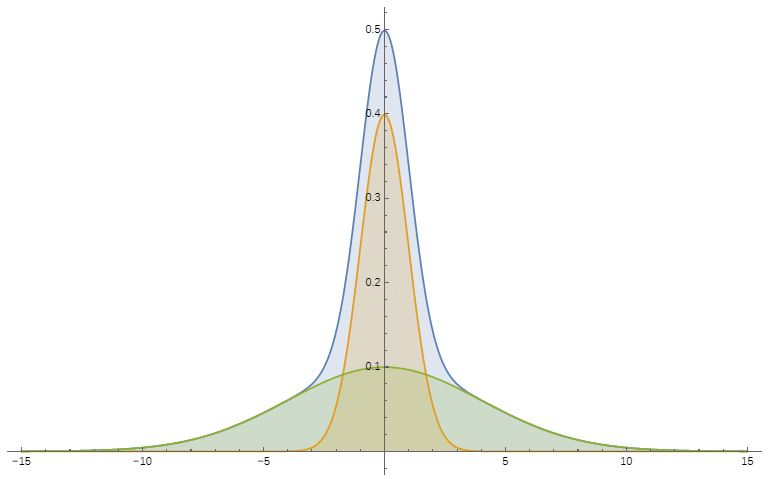
\includegraphics[width=.7\textwidth]{images/gaussians.JPG}
    \caption{Combination of two Gaussian functions.}
    \label{img:gaussTwo}
\end{figure}

In our system, we first generate each Gaussian separately using the Equation \ref{eq:bigaus}. The standard deviations of the diffuse Gaussian are set by the user in the configuration using $sigmaX$ and $sigmaY$. For the sharp Gaussian user defines parameter $sigmaFactor$ and standard deviations are calculated using Equation \ref{eq:sigmaGalaxy} mentioned in the previous chapter. The position ($x_0$,$y_0$) is the same for both Gaussians as well the rotation $\theta$. After both Gaussians are generated, the pixel values of both images are normalized into the interval <0,1>. 

In the configuration, the user defines the $brightness$ of the galaxy, more specifically the intensity of the inner core. The user also specifies the brightness of the diffuse Gaussian in a form of using $brightnessFactor$, and the brightness is calculated using Equation \ref{eq:brightnessGalaxy} from the previous chapter. 
To account for two Gaussians being added together, the sharp Gaussian has the intensity of $(1 - brightnessFactor) \cdot brightness$ and the diffuse Gaussian has $brightnessFactor \cdot brightness$ intensity. After adding the functions together, the intensity of the core is $brightness$ as defined in the configuration. 

The final galaxy profile is generated using following linear combination of Gaussians:
\begin{equation}
    galaxy = A \cdot sharpGauss + B \cdot diffuseGauss
\end{equation}
where $A$ is $(1 - brightnessFactor) \cdot brightness$ and $B$ is $brightnessFactor \cdot brightness$. 

At the end, when the galaxy is generated, Poisson noise is applied, pixel values are clipped to the interval <0,65535> and the image is added to the input image the same way as with the point and streak source. 

Again, to compare generated galaxy using the following process to a real elliptical galaxy we have created a side-by-side view of their 3D profiles in the Figure \ref{fig:galaxy3D}.

\begin{figure}[!h]
\centering
    \begin{subfigure}[t]{.4\textwidth}
        \centering
        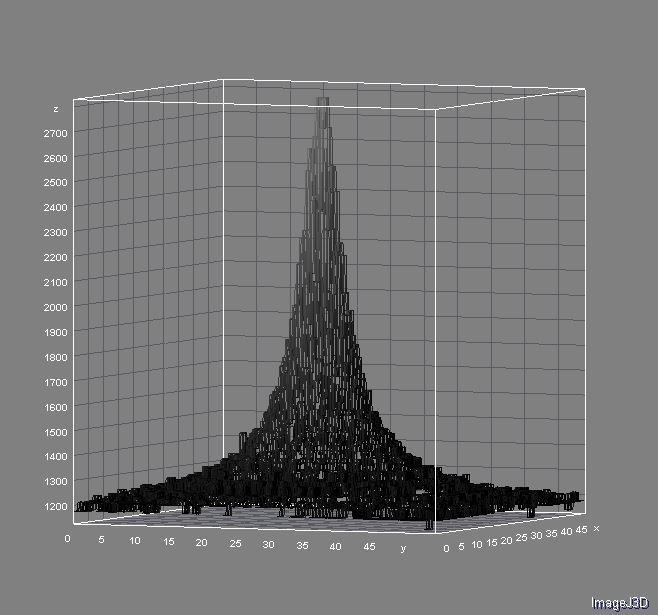
\includegraphics[width=\textwidth]{images/realGalaxy3D.JPG}
        \caption{3D profile of the real galaxy.}
        \label{fig:galaxy3D1}
    \end{subfigure}
    \begin{subfigure}[t]{.4\textwidth}
        \centering
        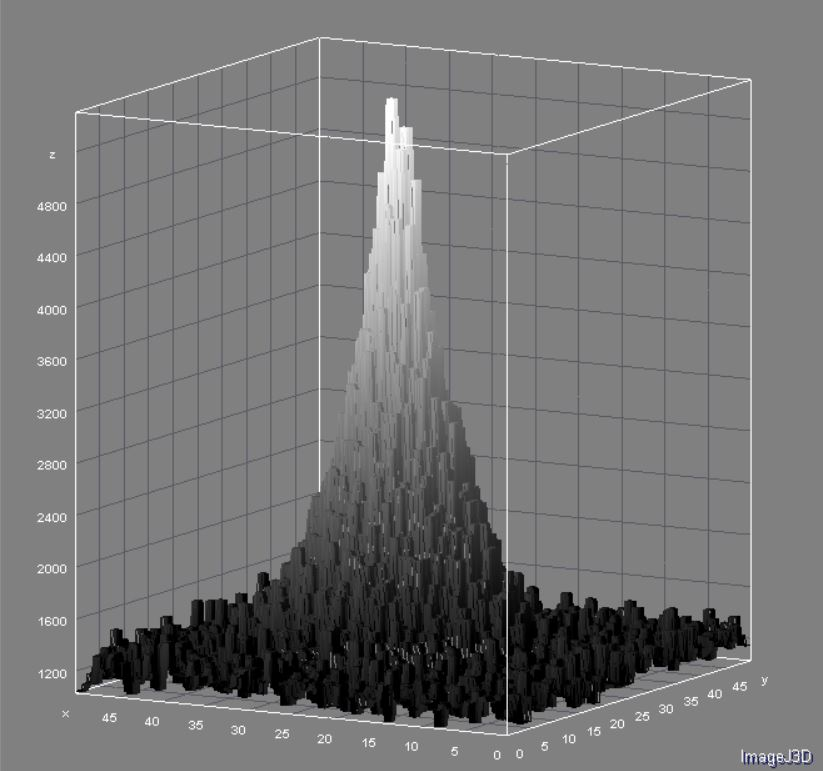
\includegraphics[width=\textwidth]{images/syngalaxy3D2.JPG}
        \caption{3D profile of the synthetic galaxy.}
        \label{fig:galaxy3D2}
    \end{subfigure}

    \caption{Comparison of 3D profiles between real and synthetic galaxies.}
    \label{fig:galaxy3D}
\end{figure}

With galaxy we have wider range of parameters to control. With $sigmaFactor$ it proved to be the best to use values ranging from 0.2 to 0.4 and with $brightnessFactor$ values from 0.6 to 0.8. In the Figure \ref{fig:galaxypar} we show how other parameters like $sigmaX$, $sigmaY$ and $alpha$ affect the generated galaxy. All images have $sigmaFactor$ set as 0.3, and $brightnessFactor$ to 0.6.  


\begin{figure}[!h]
\centering
    \begin{subfigure}[t]{.23\textwidth}
        \centering
        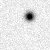
\includegraphics[width=\textwidth]{images/galaxyA.png}
        \caption{sigmaX = 3, sigmaY = 3, alpha = 0.}
        \label{fig:galaxyA}
    \end{subfigure}
    \begin{subfigure}[t]{.23\textwidth}
        \centering
        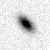
\includegraphics[width=\textwidth]{images/galaxyB.png}
        \caption{sigmaX = 3.5, sigmaY = 6.5, alpha = 135.}
        \label{fig:galaxyB}
    \end{subfigure}
    \begin{subfigure}[t]{.23\textwidth}
        \centering
        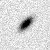
\includegraphics[width=\textwidth]{images/galaxyC.png}
        \caption{sigmaX = 5.5, sigmaY = 2.5, alpha = 45.}
        \label{fig:galaxyC}
    \end{subfigure}
    \begin{subfigure}[t]{.23\textwidth}
        \centering
        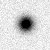
\includegraphics[width=\textwidth]{images/galaxyD.png}
        \caption{sigmaX = 5, sigmaY = 5, alpha = 0.}
        \label{fig:galaxyD}
    \end{subfigure}

    \caption{Generated images of galaxy with different values of sigmaX, sigmaY and alpha.}
    \label{fig:galaxypar}
\end{figure}

\subsection{Hot pixels}
Hot pixels are just individual pixels with very high brightness and they are generated as such. The user defines their brightness and count in the configuration. Another added parameter is that he can specify the value of the random seed which will be used when generating their positions since hot pixels are in the same position in each frame in the series. This way the system can generate multiple series with the same set of hot pixels. For the purpose of generating data for the network, we added an option to generate random positions for each series since we want to have the pixel at different locations of the image. Examples of generated hot pixels at different locations are shown in the Figure \ref{fig:hotpixelspar}.

\begin{figure}[!h]
\centering
    \begin{subfigure}[t]{.23\textwidth}
        \centering
        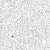
\includegraphics[width=\textwidth]{images/hotpixelA.png}
    \end{subfigure}
    \begin{subfigure}[t]{.23\textwidth}
        \centering
        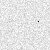
\includegraphics[width=\textwidth]{images/hotpixelB.png}
    \end{subfigure}
    \begin{subfigure}[t]{.23\textwidth}
        \centering
        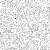
\includegraphics[width=\textwidth]{images/hotpixelC.png}
    \end{subfigure}
    \begin{subfigure}[t]{.23\textwidth}
        \centering
        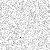
\includegraphics[width=\textwidth]{images/hotpixelD.png}
    \end{subfigure}

    \caption{Generated images of hot pixels at different positions in the image. }
    \label{fig:hotpixelspar}
\end{figure}

\subsection{Cosmic rays}
Cosmic rays can be grouped into three categories based on their appearance on the image: spots, worms, and tracks. Each type is generated separately with a different algorithm. 

Let's first consider spots. As the name suggests they resemble small spots on the image, that have very high brightness compared to the background. They are generated using an iterative method. First, the random position on the image is selected and the brightness value is assigned to it. Then another pixel is chosen from the four-neighborhood of the previous pixel and assigned a different brightness value. This continues until we create a spot with an exact number of pixels as was defined in the configuration. If the chosen neighboring pixel has already brightness assigned to it then another pixel is chosen. In the Figure \ref{fig:spotsPar} we show some examples of generated spots. 
\begin{figure}[!h]
\centering
    \begin{subfigure}[t]{.23\textwidth}
        \centering
        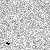
\includegraphics[width=\textwidth]{images/spotA.png}
    \end{subfigure}
    \begin{subfigure}[t]{.23\textwidth}
        \centering
        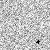
\includegraphics[width=\textwidth]{images/spotB.png}
    \end{subfigure}
    \begin{subfigure}[t]{.23\textwidth}
        \centering
        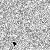
\includegraphics[width=\textwidth]{images/spotC.png}
    \end{subfigure}
    \begin{subfigure}[t]{.23\textwidth}
        \centering
        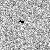
\includegraphics[width=\textwidth]{images/spotD.png}
    \end{subfigure}

    \caption{Generated images of cosmic rays - spots. }
    \label{fig:spotsPar}
\end{figure}

On the other hand, worms have a structure of a curved polyline. They are also generated using an iterative algorithm. First, we select a random position on the image and direction from 8 directions shown in the Figure \ref{img:8directions}. We move in this direction for a few pixels and fill each pixel on the way. Then another direction is selected, but it needs to differ from the previous direction only by one. So for example, if the previous direction was 8 then the next direction can be 7 or 1. This continues until we create a worm with the number of pixels defined from the configuration. Examples of some generated worms are depicted in the Figure \ref{fig:wormspar}. 

\begin{figure}[h]
    \centering
    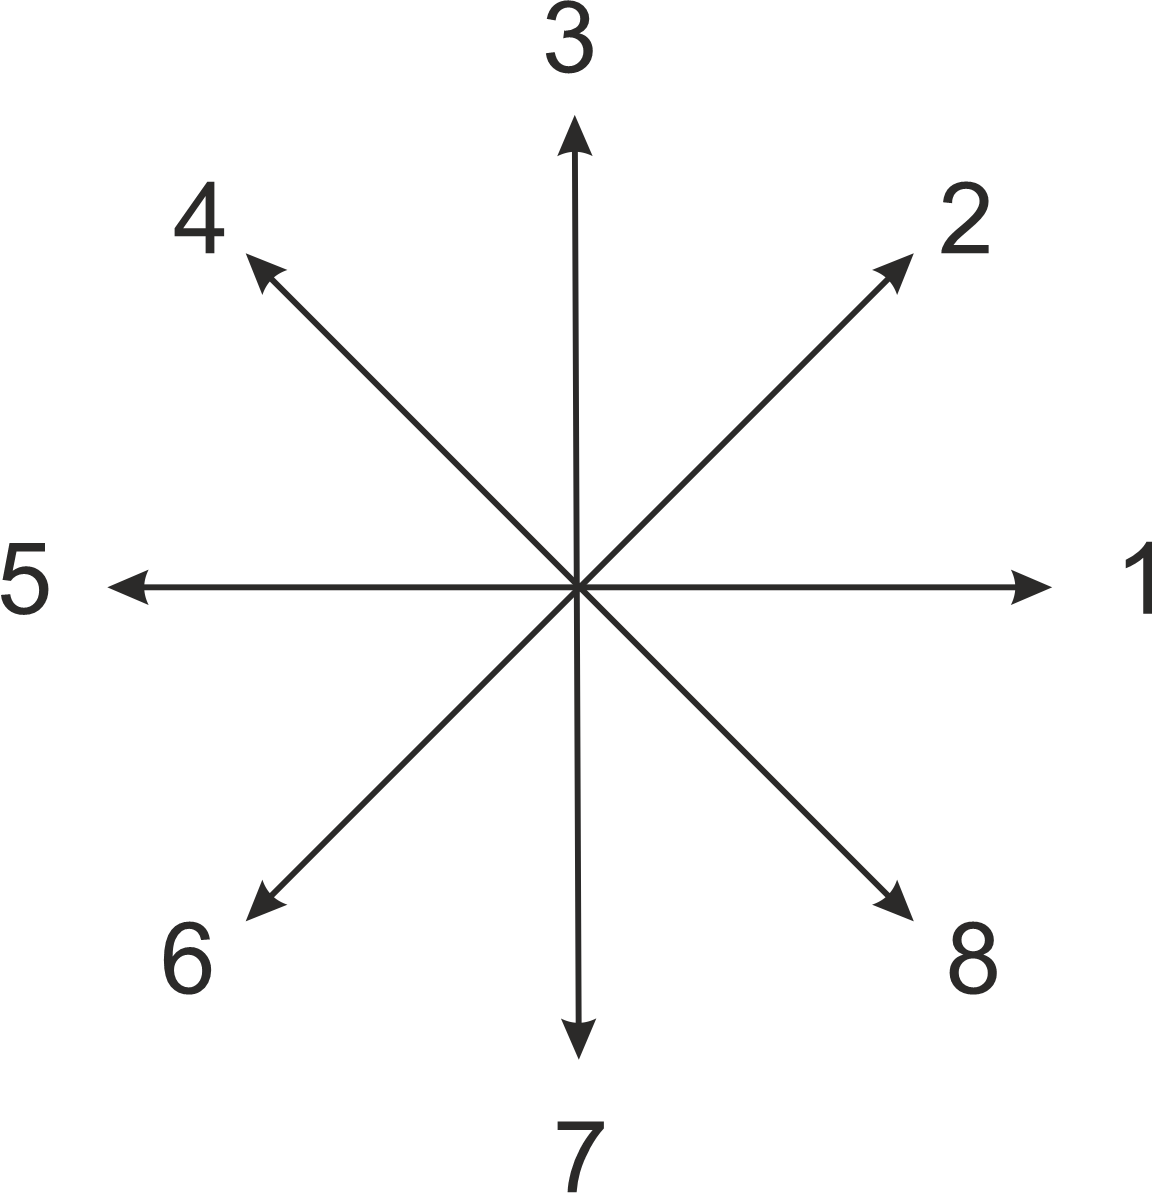
\includegraphics[width=.23\textwidth]{images/8directions.png}
    \caption{Diagram of 8 directions.}
    \label{img:8directions}
\end{figure}

\begin{figure}[!h]
\centering
    \begin{subfigure}[t]{.23\textwidth}
        \centering
        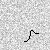
\includegraphics[width=\textwidth]{images/wormA.png}
    \end{subfigure}
    \begin{subfigure}[t]{.23\textwidth}
        \centering
        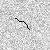
\includegraphics[width=\textwidth]{images/wormB.png}
    \end{subfigure}
    \begin{subfigure}[t]{.23\textwidth}
        \centering
        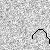
\includegraphics[width=\textwidth]{images/wormC.png}
    \end{subfigure}
    \begin{subfigure}[t]{.23\textwidth}
        \centering
        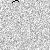
\includegraphics[width=\textwidth]{images/wormD.png}
    \end{subfigure}

    \caption{Generated images of cosmic rays - worms. }
    \label{fig:wormspar}
\end{figure}

Tracks resemble lines on the image, but generating just diagonal pixels to create them is not ideal, since tracks in real observations don't follow the precise shape of lines. The process of generating them is very similar to generating worms, with just one modification. Instead of choosing another direction every time, we establish two directions at the beginning and only follow these two. Again these two directions need to differ only by one number from the diagram of directions (Figure \ref{img:8directions}). This creates pseudo-lines as shown in the Figure \ref{fig:trackspar} where we generated some examples of tracks. 

\begin{figure}[!h]
\centering
    \begin{subfigure}[t]{.23\textwidth}
        \centering
        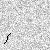
\includegraphics[width=\textwidth]{images/trackA.png}
    \end{subfigure}
    \begin{subfigure}[t]{.23\textwidth}
        \centering
        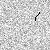
\includegraphics[width=\textwidth]{images/trackB.png}
    \end{subfigure}
    \begin{subfigure}[t]{.23\textwidth}
        \centering
        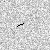
\includegraphics[width=\textwidth]{images/trackC.png}
    \end{subfigure}
    \begin{subfigure}[t]{.23\textwidth}
        \centering
        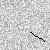
\includegraphics[width=\textwidth]{images/trackD.png}
    \end{subfigure}

    \caption{Generated images of cosmic rays - tracks. }
    \label{fig:trackspar}
\end{figure}
